\section{Implementation}
\thispagestyle{plain}

\subsection{Backlog}

Out backlog changed a lot during the project. About halfway in, we was introduced to many new requirements from our customer Jaqueline Floch. We received a list where she had written down all her requirements in priorities for the project. This list was used during the acceptance testing and can be found in section \ref{sec:TestExecution} ordered by priority. This introduction also altered the priorities a bit, but was helpful as it made our customers wishes clearer after the unfortunate start of the project.

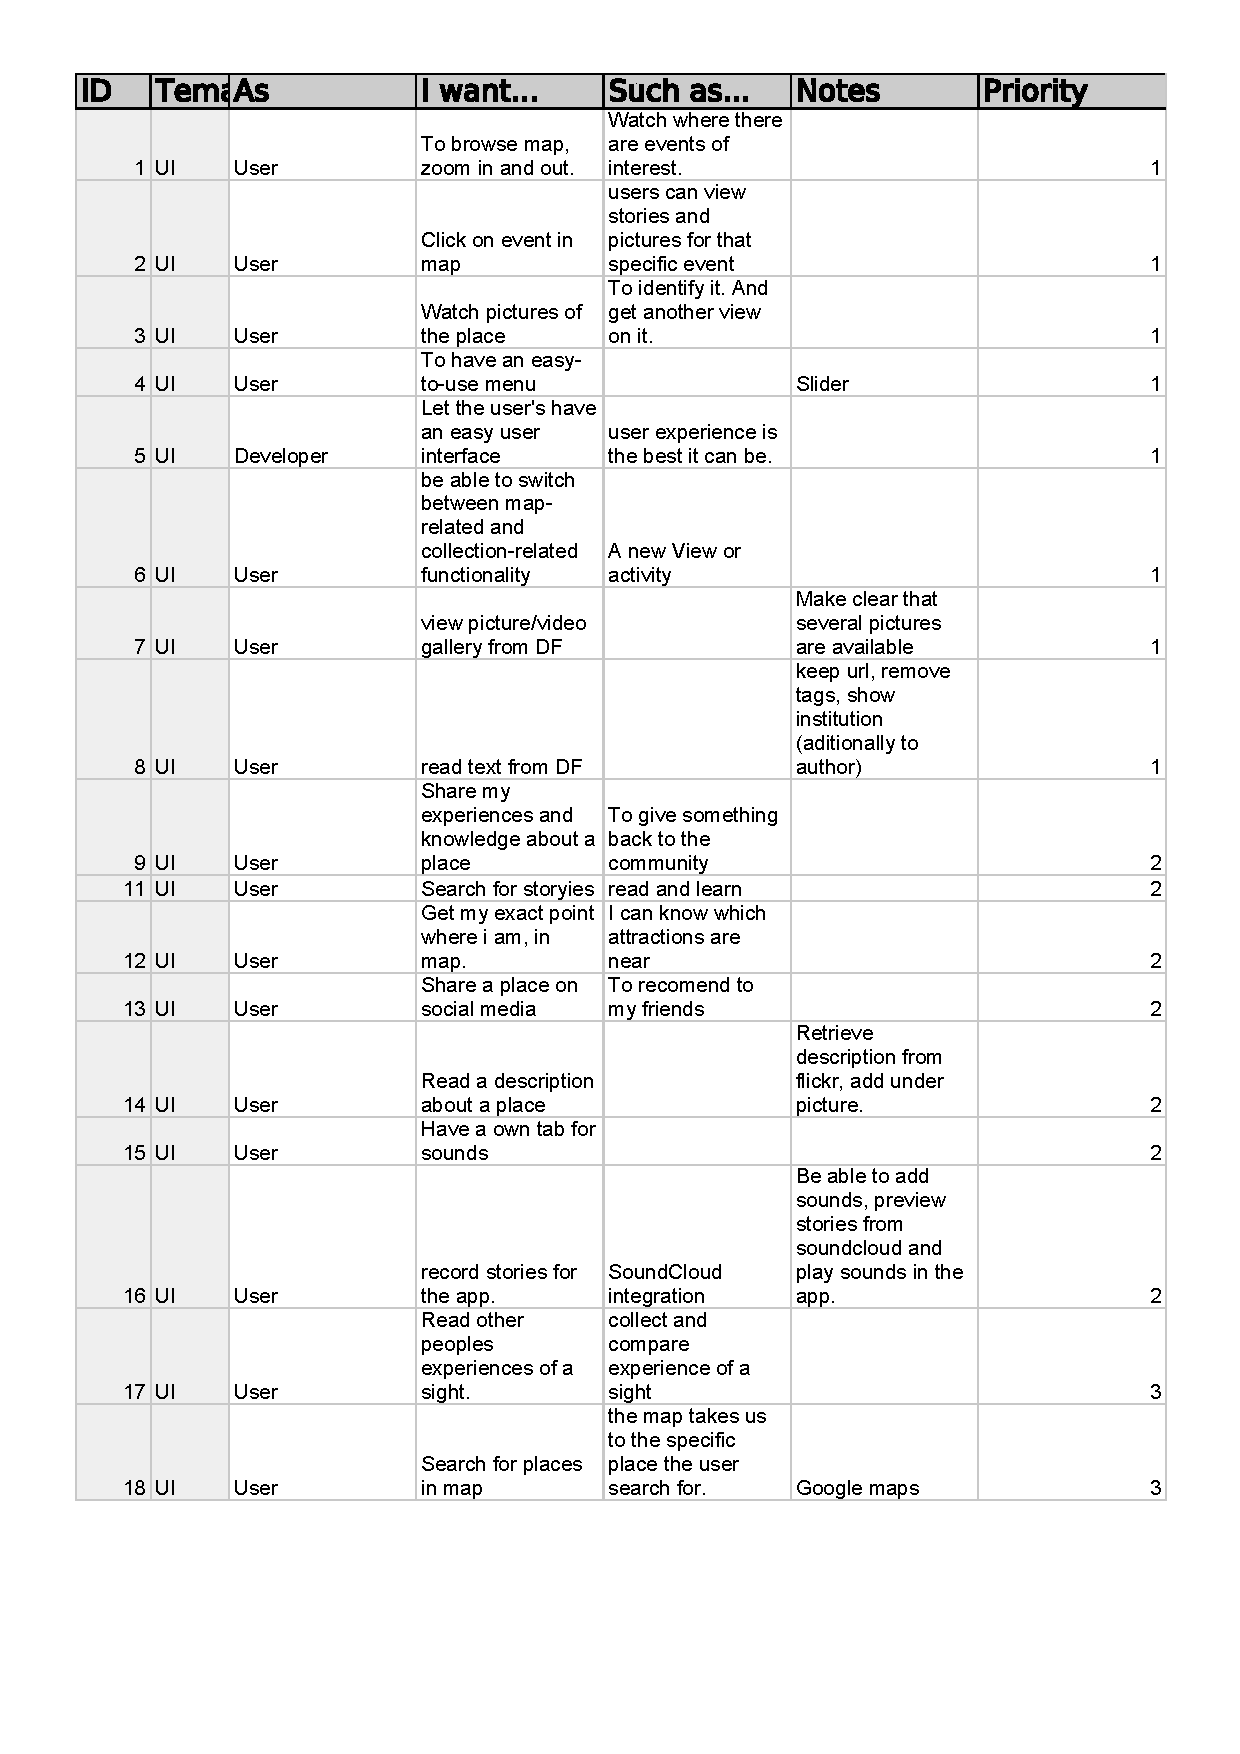
\includepdf[%
 	pages={-},
	offset=0in 0in,%
%	pagecommand={\pagestyle{fancy}},
%	pagecommand={ \pagenumbering{gobble}}
]{res/Backlog.pdf}


\subsection{Sprints}

In our version of Scrum we had two week sprints composed of entries from the sprint backlog, and was completed like descried in section \ref{sec:scrumPlanning}.
All the sprints are documented in detail in the sheet below.
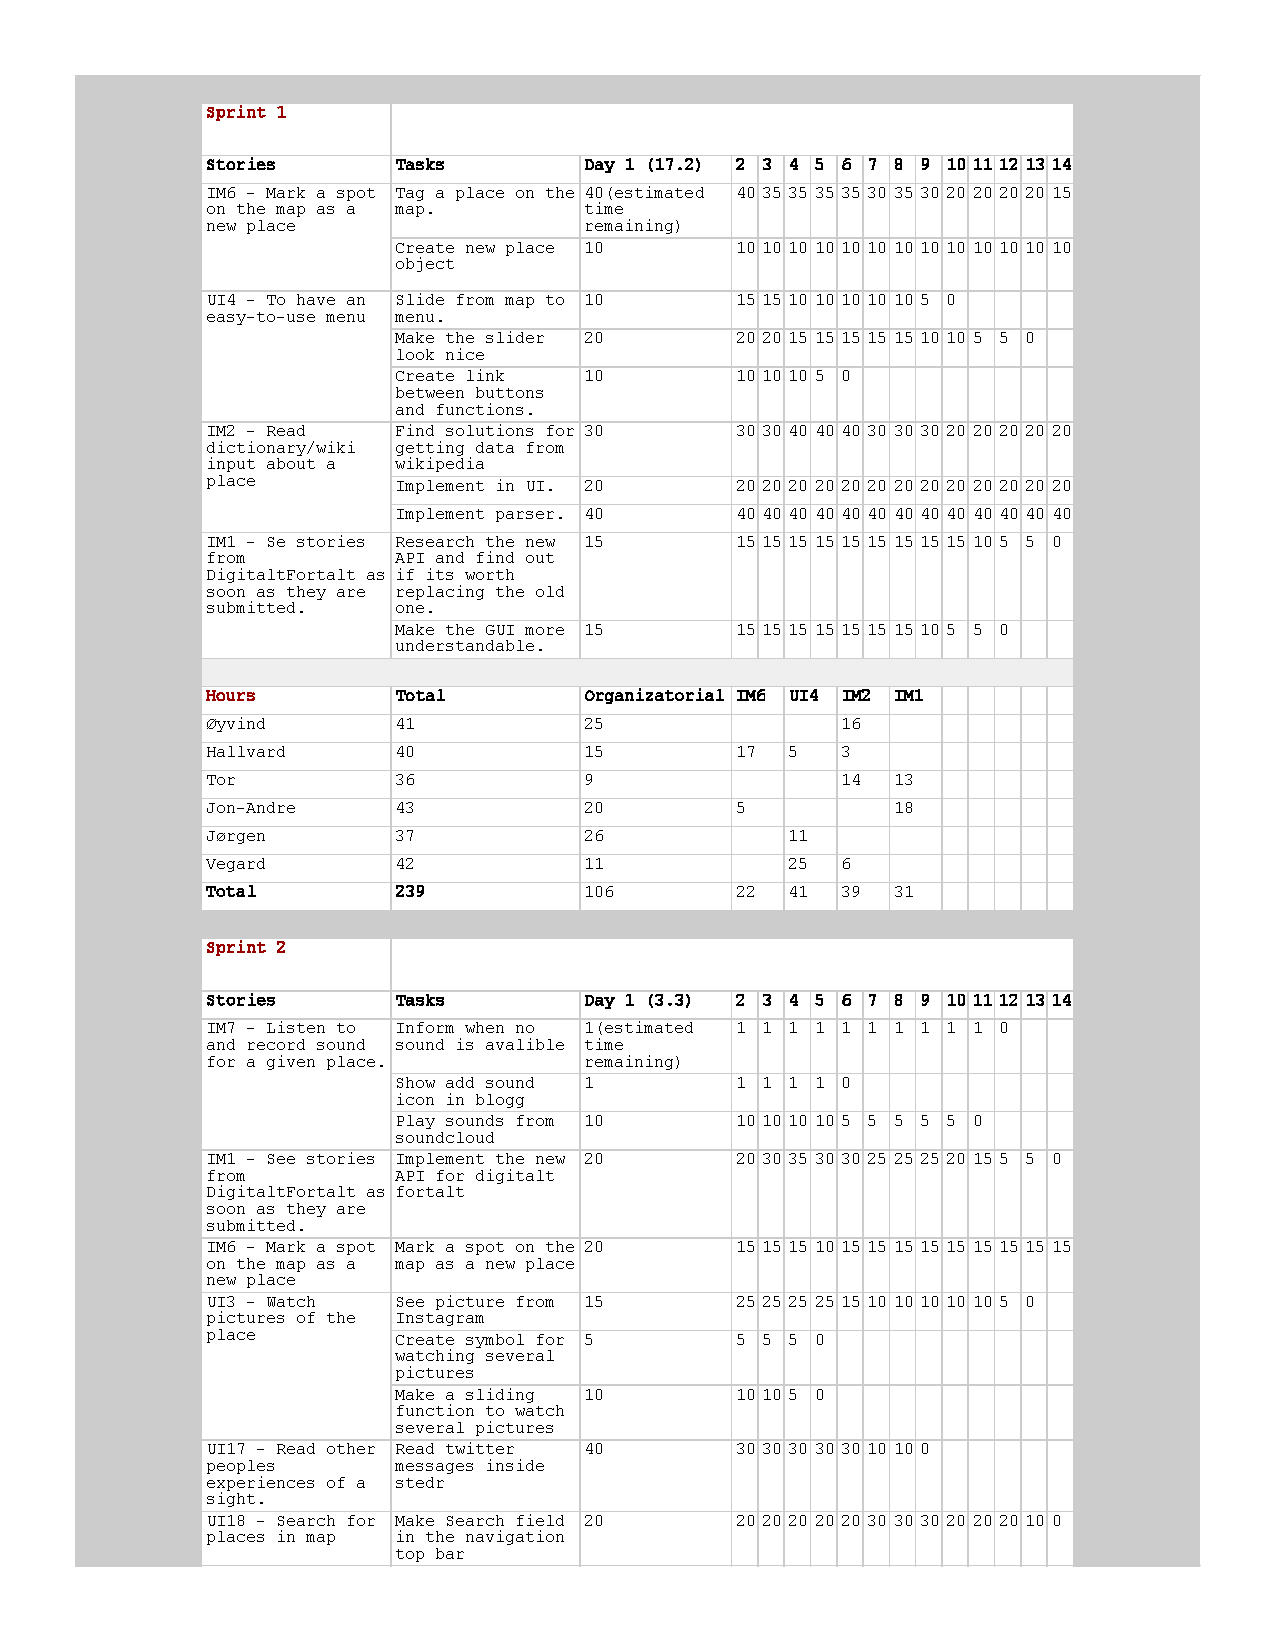
\includepdf[%
	scale=1.05,
 	pages={-},
	offset=0in -0.5in,%
	pagecommand={\pagestyle{fancy}}
]{res/Sprints.pdf}




